\pdfoutput=1
\pdfcompresslevel=9
\pdfinfo
{
    /Author ()
    /Title ()
    /Subject ()
    /Keywords ()
}

\batchmode
\nonstopmode

%\newcommand*{\memfontfamily}{pnc}
%\newcommand*{\memfontpack}{newcent}
\documentclass[a4paper,onecolumn,oneside,12pt]{memoir}
% Wydruk do archiwum
%\documentclass[a4paper,onecolumn,twoside,10pt]{memoir} 
%\renewcommand{\normalsize}{\fontsize{8pt}{10pt}\selectfont}
\usepackage[utf8]{inputenc}
\usepackage[T1]{fontenc}
\usepackage{setspace}
\usepackage{tabularx}
\usepackage{color,calc}
%\usepackage{soul} % pakiet z komendami do podkreślania tekstu
\usepackage{times} % pakiet zmieniający czcionki na times 

%\usepackage{longtable}
%\usepackage{ltxtable}
%\usepackage{tabulary}

\usepackage{indentfirst}
\usepackage{multicol}
\usepackage{listings}
\lstset{basicstyle=\footnotesize\ttfamily,breaklines=true}

%%%%%% Ustawienia odpowiedzialne za sposób łamania dokumentu
%\hyphenpenalty=10000		% nie dziel wyrazów zbyt często
\clubpenalty=10000      %kara za sierotki
\widowpenalty=10000  % nie pozostawiaj wdów
\brokenpenalty=10000		% nie dziel wyrazów między stronami
\exhyphenpenalty=999999		% nie dziel słów z myślnikiem
\righthyphenmin=3			% dziel minimum 3 litery

%\tolerance=4500
%\pretolerance=250
%\hfuzz=1.5pt
%\hbadness=1450

%ustawienia rozmiarów: tekstu, stopki, marginesów 
\setlength{\textwidth}{\paperwidth}
\addtolength{\textwidth}{-5cm}
\setlength{\textheight}{\paperheight}
\addtolength{\textheight}{-5cm}
\setlength{\oddsidemargin}{-0.04cm} % domyślnie jest 1 cal = 2.54 cm, stąd -0.04 da margines 2.5cm
\setlength{\evensidemargin}{-0.04cm} % domyślnie jest 1 cal = 2.54 cm, stąd -0.04 da margines 2.5cm
\topmargin -1.25cm 
\footskip 1.4cm 

\linespread{1}
%\linespread{1.3}

\usepackage{ifpdf}
%\newif\ifpdf \ifx\pdfoutput\undefined
%\pdffalse % we are not running PDFLaTeX
%\else
%\pdfoutput=1 % we are running PDFLaTeX
%\pdftrue \fi
\ifpdf
\usepackage[pdftex]{graphicx,hyperref}
\DeclareGraphicsExtensions{.pdf,.jpg,.mps,.png}
\pdfcompresslevel=9
\else
\usepackage{graphicx}
\DeclareGraphicsExtensions{.eps,.ps,.jpg,.mps,.png}
\fi
\sloppy

%\graphicspath{{rys01/}{rys02/}}
%\usepackage{rotating}

\renewcommand{\topfraction}{1.0}
\renewcommand{\bottomfraction}{1.0}
\renewcommand{\textfraction}{0.0}
\renewcommand{\floatpagefraction}{0.35}

%%%%%%%%%%%%%%%%%%%%%%%%%%%%%%%%%%%%%%%
%                  Definicja strony tytułowej 
%%%%%%%%%%%%%%%%%%%%%%%%%%%%%%%%%%%%%%%
\makeatletter
%Uczelnia
\newcommand\uczelnia[1]{\renewcommand\@uczelnia{#1}}
\newcommand\@uczelnia{}
%Wydział
\newcommand\wydzial[1]{\renewcommand\@wydzial{#1}}
\newcommand\@wydzial{}
%Kierunek
\newcommand\kierunek[1]{\renewcommand\@kierunek{#1}}
\newcommand\@kierunek{}
%Specjalność
\newcommand\specjalnosc[1]{\renewcommand\@specjalnosc{#1}}
\newcommand\@specjalnosc{}
%Tytuł po angielsku
\newcommand\titleEN[1]{\renewcommand\@titleEN{#1}}
\newcommand\@titleEN{}
%Tytuł krótki
\newcommand\titleShort[1]{\renewcommand\@titleShort{#1}}
\newcommand\@titleShort{}
%Promotor
\newcommand\promotor[1]{\renewcommand\@promotor{#1}}
\newcommand\@promotor{}

\def\maketitle{%
  \null
  \pagestyle{empty}%
	{\centering\vspace{-1cm}
		{\fontsize{22pt}{24pt}\selectfont \@uczelnia}\\[0.4cm]
		{\fontsize{22pt}{24pt}\selectfont \@wydzial }\\[0.5cm]
		\hrule \vspace*{0.7cm}
	}
{\flushleft\fontsize{14pt}{16pt}\selectfont%
\begin{tabular}{ll}
KIERUNEK: & \@kierunek\\
SPECJALNOŚĆ: & \@specjalnosc\\
\end{tabular}\\[1.3cm]
}
{\centering
\vskip 1cm
{\fontsize{24pt}{26pt}\selectfont PRACA DYPLOMOWA}\\[0.5cm]
{\fontsize{24pt}{26pt}\selectfont MAGISTERSKA}\\[2cm]
%{\fontsize{24pt}{26pt}\selectfont PROJEKT INżYNIERSKI}\\[1.5cm]
\vskip 0.8cm
}
%
\begin{tabularx}{\linewidth}{p{6cm}>{\centering\arraybackslash}X}
		&{\fontsize{16pt}{18pt}\selectfont \@title}\\[5mm] 	%UWAGA: tutaj jest miejsce na tytył w języku polskim
		&{\fontsize{16pt}{18pt}\selectfont \@titleEN}\\[10mm] %UWAGA: tutaj jest miejsce na tytył w języku angielskim
\end{tabularx}
\vfill
\begin{tabularx}{\linewidth}{p{6cm}l}
		%UWAGA: tutaj jest miejsce na autora pracy
		&{\fontsize{16pt}{18pt}\selectfont AUTOR:}\\[5mm]
		&{\fontsize{14pt}{16pt}\selectfont \@author}\\[10mm]
		%UWAGA: tutaj jest miejsce na promotora pracy 
		&{\fontsize{16pt}{18pt}\selectfont PROWADZĄCY PRACĘ:}\\[5mm]
		&{\fontsize{14pt}{16pt}\selectfont \@promotor}\\[10mm]
		&{\fontsize{16pt}{18pt}\selectfont OCENA PRACY:}\\[20mm]
	\end{tabularx}
\hrule\vspace*{0.3cm}
{\centering
%{\fontsize{24pt}{26pt}\selectfont PRACA DYPLOMOWA}\\[0.5cm]
%{\fontsize{24pt}{26pt}\selectfont MAGISTERSKA}\\[2cm]
{\fontsize{16pt}{18pt}\selectfont \@date}\\[0cm]
}
\normalfont
 \cleardoublepage
}
\makeatother
%%%%%%%%%%%%%%%%%%%%%%%%%%%%%%%%%%%%%%%
%                  Styl rozdziałów 
%%%%%%%%%%%%%%%%%%%%%%%%%%%%%%%%%%%%%%%
\setcounter{secnumdepth}{3}
\setcounter{tocdepth}{3}
%\definecolor{niceblue}{rgb}{.168,.234,.671}

%\AtBeginDocument{% 
%        \addto\captionspolish{% 
%        \renewcommand{\tablename}{Table}% 
%}%} 

%\AtBeginDocument{% 
%        \addto\captionspolish{% 
%        \renewcommand{\chaptername}{Rozdział}% 
%}} 

%\AtBeginDocument{% 
%        \addto\captionspolish{% 
%        \renewcommand{\figurename}{Image}% 
%}%}
%        \addto\captionspolish{% 
%        \renewcommand{\bibname}{Literature}% 
%}


%%%%%%%%%%%%%%%%%%%%%%%%%%%%%%%%%%%%% nowe itemize
\makeatletter
\renewenvironment{itemize}{
  \begin{list}{  
  \csname labelitem\romannumeral\the\@listdepth\endcsname}{
  \setlength{\leftmargin}{1em}
	\setlength{\topsep}{6pt}%
	\setlength{\partopsep}{0pt}%
	\setlength{\parskip}{0pt}%
	\setlength{\parsep}{0pt}%
	\setlength{\itemsep}{0pt}}
}{
  \end{list}
}

%%%%%%%%%%%%%%%%%%%%%%%%%%%%%%%%%%%%%%%%%%%%%%%%%%%%%%%%%%%%%%%%%% Styl wyliczenia (opis skrótów) 
%%%%%%%%%%%%%%%%%%%%%%%%%%%%%%%%%%%%%%%%%%%%%%%%%%%%%%%%%%%%%%%%%
\newenvironment{Ventry}[1]%
 {\begin{list}{}{\renewcommand{\makelabel}[1]{\textbf{##1}\hfill}%
   \settowidth{\labelwidth}{\textbf{#1}}%
   \setlength{\leftmargin}{3cm}}}%
 {\end{list}}

\addtopsmarks{headings}{%
\nouppercaseheads % added at the beginning
}{%
\createmark{chapter}{both}{shownumber}{}{. \space}
%\createmark{chapter}{left}{shownumber}{}{. \space}
\createmark{section}{right}{shownumber}{}{. \space}
}%use the new settings
\pagestyle{headings}

\newlength\mytemplengtha

\setcounter{secnumdepth}{2}
\setcounter{tocdepth}{2}
\setsecnumdepth{subsection} % activating subsubsec numbering in doc

\makeatletter
\copypagestyle{outer}{headings}
\makeoddhead{outer}{}{}{\slshape\rightmark}
\makeevenhead{outer}{\slshape\leftmark}{}{}
\makeoddfoot{outer}{\@author:~\@titleEN}{}{\thepage}
\makeevenfoot{outer}{\thepage}{}{\@author:~\@titleEN}
\makeheadrule{outer}{\linewidth}{\normalrulethickness}
\makefootrule{outer}{\linewidth}{\normalrulethickness}{6pt}
\makeatother

% fix plain
%\copypagestyle{plain}{outer} % overwrite plain with outer
\makeoddhead{plain}{}{}{} % remove right header
\makeevenhead{plain}{}{}{} % remove left header
\makeevenfoot{plain}{}{}{}
\makeoddfoot{plain}{}{}{}

%\copypagestyle{plain}{outer} % overwrite plain with outer
\makeoddhead{empty}{}{}{} % remove right header
\makeevenhead{empty}{}{}{} % remove left header
\makeevenfoot{empty}{}{}{}
\makeoddfoot{empty}{}{}{}

\pagestyle{outer}

%definicja nagłówków
%\renewcommand{\chaptermark}[1]{\markboth{\ifnum \c@secnumdepth >\z@ \thechapter \ \fi #1}{}} 
%\renewcommand{\chaptermark}[1]{\markboth{\thechapter \ #1}{\thesection \ #1}} 
%\renewcommand{\sectionmark}[1]{\markright{\thesection \ #1}{}} 
%\renewcommand{\chaptermark}[1]{\markboth{\thechapter \MakeUppercase{#1}}{}}

%kropki po numerach sekcji
\makeatletter
\def\@seccntformat#1{\csname the#1\endcsname.\quad}
\def\numberline#1{\hb@xt@\@tempdima{#1\if&#1&\else.\fi\hfil}}
\makeatother

\renewcommand{\chapternumberline}[1]{#1.\quad}
\renewcommand{\cftchapterdotsep}{\cftdotsep}

%\AtBeginDocument{\addtocontents{toc}{\protect\thispagestyle{empty}}}

%\includeonly{wstep,rozdzial01} % jeśli chcemy kompilować tylko fragmenty, to można tu je wpisać
%%%%%%%%%%%%%%%%%%%%%%%%%%%%%%%%%%%%%%%%%
%                  Początek dokumentu 
%%%%%%%%%%%%%%%%%%%%%%%%%%%%%%%%%%%%%%%%%
\begin{document}
\title{Filtracja i segmentacja drukowanych w kolorze obrazów}
\titleShort{Filtracja i segmentacja drukowanych w kolorze obrazów}
\titleEN{Preprocessing and segmentation of color-printed images}
\author{Marcin Wojciechowski}
\uczelnia{POLITECHNIKA WROCŁAWSKA}
\wydzial{WYDZIAŁ ELEKTRONIKI}
\kierunek{INFORMATYKA}
\specjalnosc{Internet Engineering}
\promotor{dr inż. Tomasz Babczyński}
\date{WROCŁAW, 2014}
\maketitle

\pagestyle{outer}
\mbox{}\pdfbookmark[0]{Table of Contents}{spisTresci.1}
\tableofcontents* 
\newpage

\chapter{Introduction}

Beginning of this chapter is focused on a problem background. Next part is a 
full description of the topic and definition of main objectives of this thesis.
Finally there is presented a full structure of this document.

\section{Background}

Nowadays image digitization is a very important topic. It has a lot of practical applications.
For example, it is a very good way to prevent destruction of old photos,
to archive them(to keep them in one place in a digital version) and make it easier to 
send it from one place to another. Unfortunately, basic method of digitization of
images - scanning - has some disadvantages. Due to errors made during a scanning procedure,
input image distortions or quality of a scanning device, resulting digitized images 
have a poor quality. To improve digitization process there are many filtration algorithms,
which task is to solve this problem and to produce an image with better quality.Image digitization 
has another big advantage - there is a possibility to retrieve information from the picture(for 
example: pattern recognition, feature extraction). This feature is handled by segmentation 
algorithms. Although this group is one of the most difficult in image processing, there is a big 
emphasis on a research, due to many advantages of this type of algorithms in practical use.

\section{Problem statement and main objectives}

The main aim of this thesis is to create a filtration and segmentation algorithm, which should
apply to scanned color-printed images. This work is focused on scanned maps. 
Resulting algorithm should be optimized to used it with this type of scanned images. 
Output image should have following properties:

\begin{itemize}
  \item most of distortions should be eliminated;
  \item image should be divided into consistent areas, like forests, lakes, rivers, etc. These areas
        should be marked on the map in a consistent way(it should have the same color);
  \item detected areas should have the same size like in an input image;
  \item small details, like text should be kept and marked in a resulting image.
\end{itemize}

Used fltering algorithms should remove main distortions and all disadvantages of image scanning(like
for example rasters, moro effect). Next, proper segmentation algorithm should be used to detect all
areas in an input map and to divide the map into different, homogenous regions. \\

The final solution - set of algorithms - should be impemented in a chosen programming language.
Created application should be tested on many different scanned maps. Test results should be then
analysed.

\section{Document structure}

This document has been divided into seven chapters and the bibliography at the end.
Below there is a short description of a content for each chapter:

% TODO do przepisania po napisaniu całości pracy. Na razie mocno nieaktualne

\begin{itemize}
  \item In a first chapter there is a description and the background of the topic, 
        next there are listed main objectives of the work and a problem statement;
  \item In a second chapter there is an analysis of existing research work and solutions
        of the problem;
  \item In a third chapter there is a theoretical introduction to the problem. There are 
        findings after analysis of input images, problems which should be taken into consideration
        and algorithm properties, which should be applied;
  \item Fourth chapter focuses on research part of this thesis. There is a full description of
        filtration and segmentation algorithms used in this work;
  \item Fifth chapter focuses on engineering part of the thesis. There is a description of 
        all implementation details of the algorithm;
  \item In a sixth chapter there are presented results of all taken tests;
  \item In a seventh chapter there are conclusions of the thesis.
\end{itemize}

\chapter{Theoretical introduction}

This section contains all needed definitions and concepts needed for a good understanding of the
work. It also covers history and basic usage of digital image processing.

\section{Digital image processing}

\subsection{History and usage}

According to \cite{digitalImageProcessing},
digital image processing has a lot of practical applications. It was used first at the beginning of
XX century to send pictures over long distances. Research and development of digital image
processing algorithms  was strongly associated with growth of the computer industry. It was caused
by high computational complexity of this type of algorithms. Further growth began in 1960s. Many 
techniques were developed in organisations like Jet Propulsion Laboratory, Massachusetts Institute
of Technology or Bell Laboratories. It was used in satellite imagery, medical imaging(in 1970s 
computerized tomography was developed), image enhancement, science(for example in geography - 
in research about pollution, archeology - in restoring blured pictures), defence or industry.
Another area of digital image processing focuses on extracting an information from the picture in
a for suitable for computer processing. It is used in a character recognition(OCR), industry(
automatic inspection of production process), military, forensics(recognition of fingerprints) and
weather prediction. \\

Nowadays, with fast computers and signal processors, digital image processing is used widely.
It is mainly caused by its low price and versatility.

\subsection{Basic definitions}

A digital image can be defined as a two dimentional function f(x, y), where x and y denote spatial 
coordinates and f(x, y) is the intensity or gray level of the image at this point. Values of x, y
and f(x, y) should be finite, descrete quantities. Digital image processing refers to processing 
digital images by means of a digital computer. It includes many primitive operations like noise
reduction, contrast enhancement or image sharpening. It also involves more advanced algorithms like
image segmentation(partitioning an image into regions or objects), description of objects,
classification(recognition) of objects and even advanced analysis of an image. Digital image 
processing algorithms take an image as an input. Output depends on a type of the algorithm.
It can be new, processed image or group of attributes taken from an image. Main tasks of digital
image processing are:

\begin{itemize}
  \item Image aquisition;
  \item Image enhancement;
  \item Image restoration;
  \item Wavelets;
  \item Compression;
  \item Feature extraction;
  \item Segmentation;
  \item Recognition.
\end{itemize}

This work focuses mainly on image enhancement and image segmentation. All algorithms used in this 
work are described in next sections.

\section{Image enhancement}

Image enhancement algorithms are one of the simplest and most commonly used group of digital image
processing. Main idea of these algorithms is to improve image quality, bring out obscured details 
or highlight certain features of an image.  The main aim of image enhancement is to process image 
and return an image more suitable, than input for a specific application. Proper image enhancement
algorithms should be chosen for different cases(algorithm solving one problem may be inadequate for
other problems). Image enhancement algorithms can be divided into two groups:

\begin{itemize}
  \item Spatial domain - manipulation of pixels of an image directly;
  \item Frequency domain - modification of Fourier transform of an image.
\end{itemize}

\subsection{Smoothing algorithms}

According to \cite{learningOpenCv}, smoothing is a very simple and frequently used operation. It is
used to reduce noise or camera artifacts. It is also used in an image resolution reduction. In this
work, there are two smoothing algorithms used.

\subsubsection{Gaussian blur}

Gaussian filter is one of the most frequently used filters. According to \cite{learningOpenCv}, 
gaussian blur is done by convolving each point in the input array with a Gaussian kernel and then
summing to produce the output array. Resulting image is a smooth blur. It is used to reduce noise
or image details and as a part of edge detection algorithms. Example result of a Gaussian Blur
filter is shown in a Fig.~\ref{gaussianBlurExample}.

\begin{figure}[ht]
\begin{center}
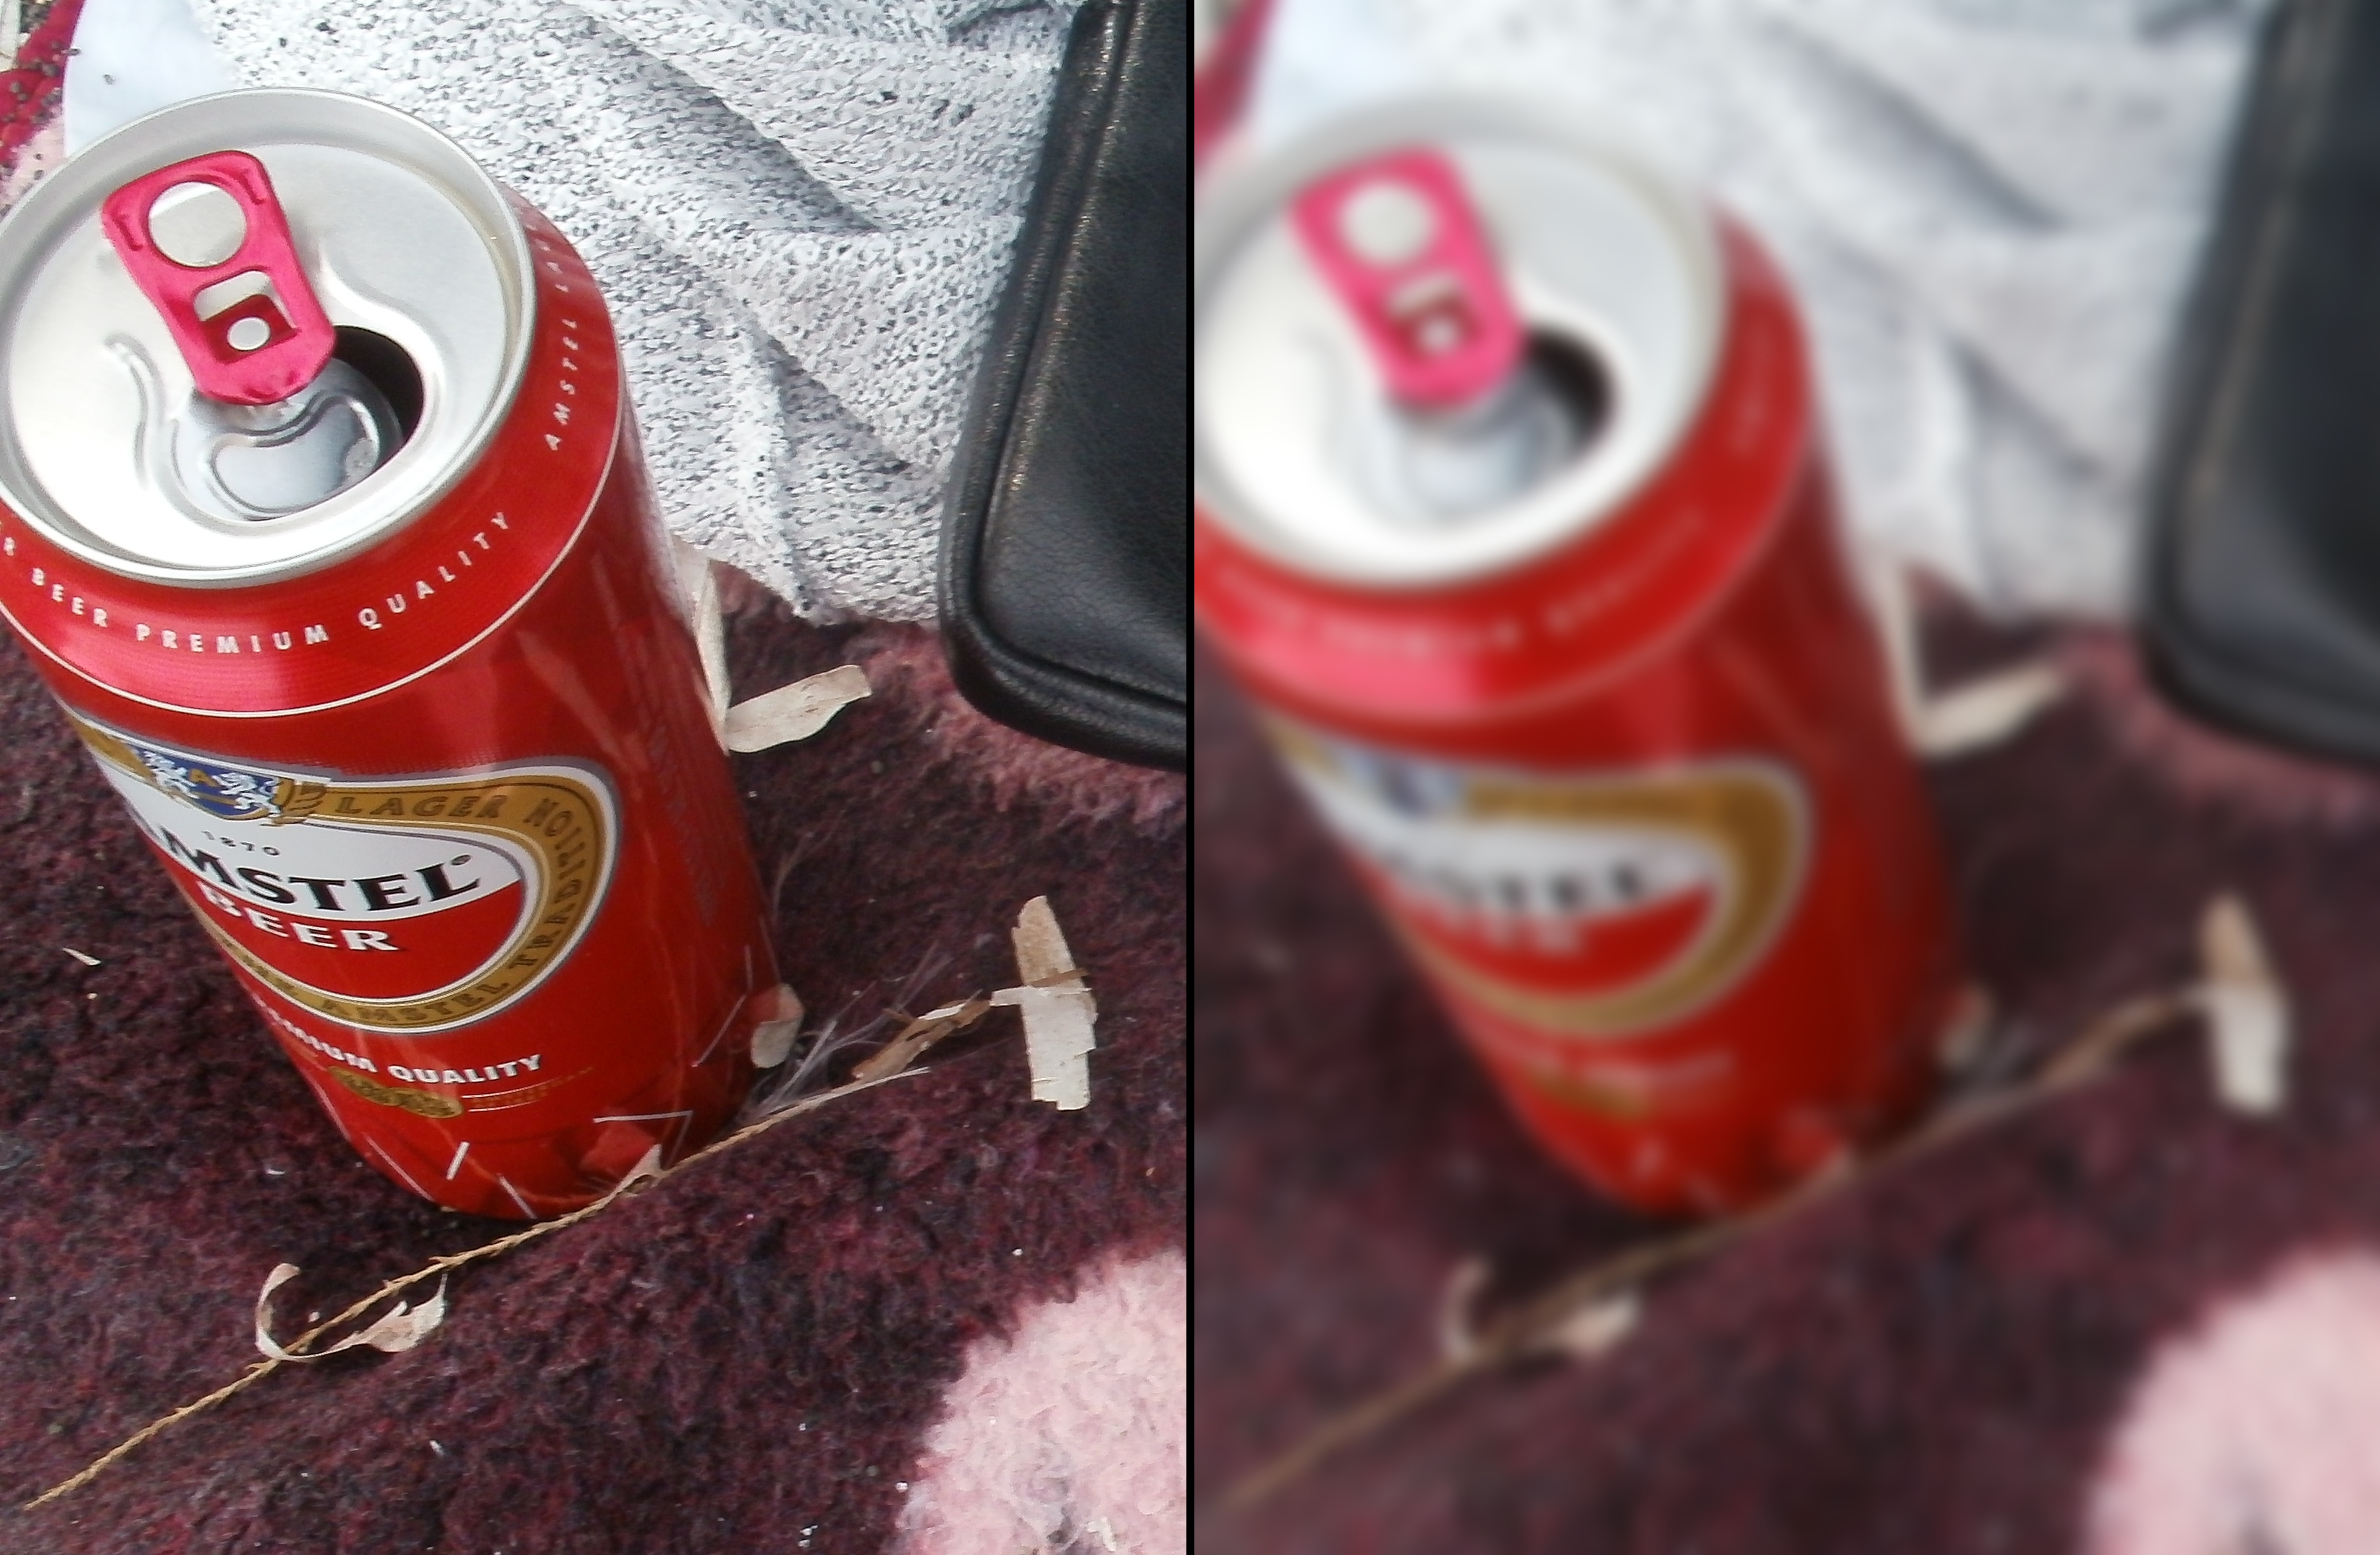
\includegraphics[scale=1.0]{images/GaussianBlurExample.jpg}
\caption{Gaussian Blur example. \\
Source: http://en.wikipedia.org/wiki/File:Halftone,\_Gaussian\_Blur.jpg}
\label{gaussianBlurExample}
\end{center}
\end{figure}

\subsubsection{Bilateral filter}

According to \cite{bilateralFilterWiki}, bilateral filter is a non-linear, edge-preserving and
noise reducing filter for images. The intensity value at each pixel in an image is replaced by a
weighted average of an intensity values from nearby pixels. In contrast to the Gaussian Blur, 
weights are based on the difference of intensity from the center pixel. This algorithm is commonly
used to prepare an input for segmenting algorithms. Example of a bilateral filter usage is presented
in a fig.~\ref{bilateralFilterExample}.

\begin{figure}[ht]
\begin{center}
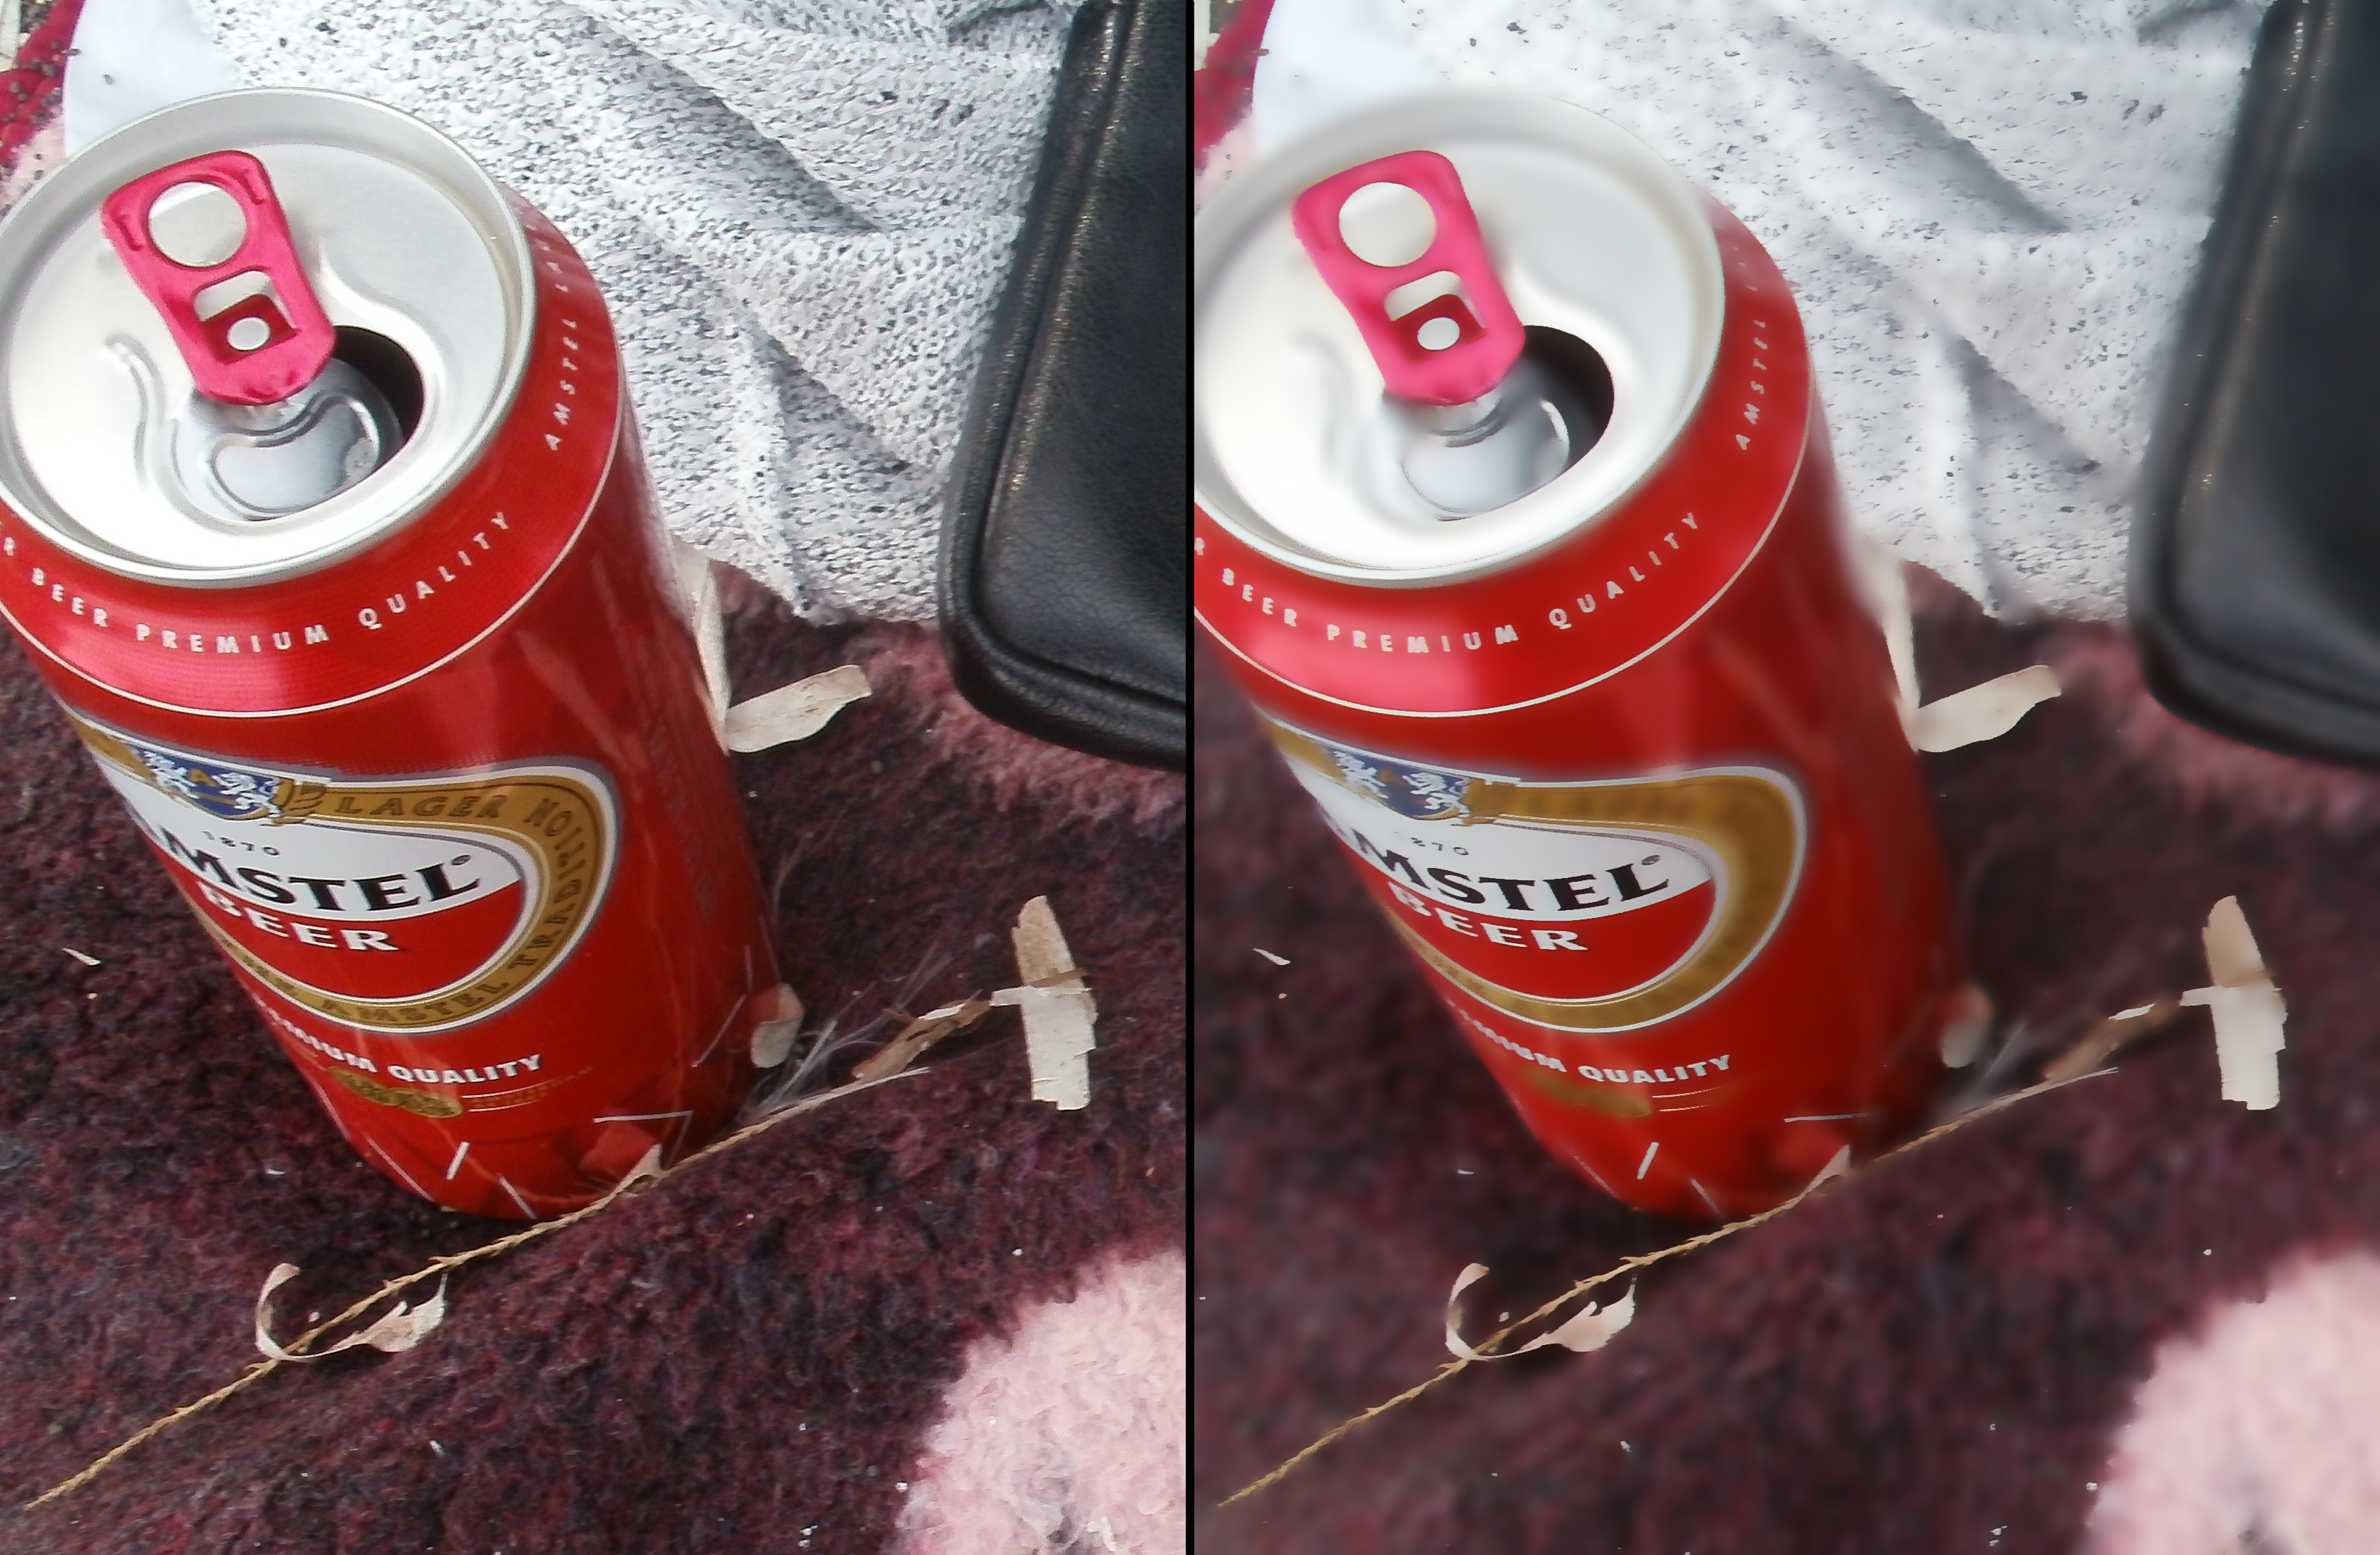
\includegraphics[scale=0.6]{images/BilateralFilterExample.jpg}
\caption{Bilateral Filter example. \\
Source: http://www.planet-source-code.com/Upload\_PSC/ScreenShots/PIC20103161922506817.jpg}
\label{bilateralFilterExample}
\end{center}
\end{figure}

\subsection{Morphological transformations}

Morphological operations are used to remove noise, isolate or joining disparate elements
in an image and find intensity bumps or holes in an image to find image gradients. Basic 
morphological operations are called Dilation and Erosion.

\subsubsection{Dilation}

Dilation is a convolution of an image with a kernel. The kernel can have any shape or size and has
to have defined an anchor point. When kernel is scanned over the image, there is computed maximum
pixel value covered by the kernel. Then, the anchor point value is set to maximum value. Dilation
causes growth of all bright elements in an image. Example of dilation is presented in 
Fig.~\ref{dilationExample}

\begin{figure}[ht]
\begin{center}
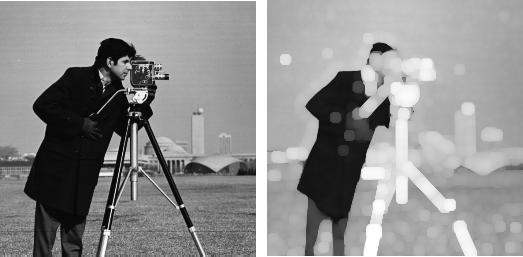
\includegraphics[scale=0.6]{images/dilationExample.jpg}
\caption{Dilation example. \\
Source: http://www.mathworks.com/help/images/ref/referenceipart130.gif}
\label{dilationExample}
\end{center}
\end{figure}

\subsubsection{Erosion}

Erosion is a converse operation to dilation. Main difference is that it computes local minimum over
the area of the kernel. Erosion causes growth of all dark elements in an image. Example of erosion
is presented in Fig.~\ref{erosionExample}

\begin{figure}[ht]
\begin{center}
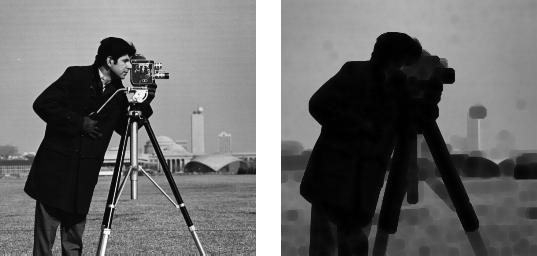
\includegraphics[scale=0.6]{images/erosionExample.jpg}
\caption{Erosion example. \\
Source: http://www.mathworks.com/help/images/ref/referenceipart128.gif}
\label{erosionExample}
\end{center}
\end{figure}

\subsection{Noise elimination}

Opis...

\subsection{Unsharp mask}

Unsharp mask is applied to highlight or enhance some details in an image. There are many 
implementations of unsharp algorithms. Depending on the application, other algorithm is used.

\section{Image segmentation}

Segmentation algorithms partitions images into constituent parts or objects. I dalsza część opisu...

\subsection{Tresholding}

Opis...



\chapter{State of Art}

This chapter focuses on actual research in topic of filtration and segmentation of scanned color
images. There is also a description of basic filtration and segmentation algorithms used in this
work.

\section{Digital image processing}

\section{Processing color scanned maps}

\section{Conclusion}


\chapter{Research design}

\section{Input data description}

\section{Problems and restrictions}

\section{Main parts of the algorithm}

\section{Detection of areas}

\section{Detection of smaller elements}

\section{Merge of layers}

\section{Conclusion}


\chapter{Implementation of the algorithm}

\section{Introduction}

\section{Used tools}

\section{Application outline}

\section{Conclusion}


\chapter{Tests and Results}

\section{Test description}

\section{Result analysis}

\section{Conclusion}


\chapter{Conclusion}

\newpage

\begin{thebibliography}{   }

	\bibitem{digitalImageProcessing}
          {Rafael C. Gonzalez, E. Woods, Digital Image Processing, Prentice Hall, 3rd Edition, 2007}
  \bibitem{learningOpenCv}
          {Gary Bradski, Adrian Kaehler, Learning OpenCV. Computer Vision with the OpenCV Library,
          O`Reilly Media Inc., 2008}
  \bibitem{bilateralFilterWiki}
          {http://en.wikipedia.org/wiki/Bilateral\_filter, Version from 29.05.2014}


\end{thebibliography}

\end{document}
